\documentclass[12pt]{article}
\usepackage[utf8]{inputenc}
\usepackage[spanish]{babel}
%\usepackage[spanish]{babel}
%\usepackage[T1]{fontenc}
%\usepackage{dejavu}
\usepackage{enumitem}
\usepackage[table,xcdraw]{xcolor}

\usepackage{listings}
\usepackage{amsfonts}
\usepackage{fancyhdr}
\usepackage{comment}
\usepackage{graphicx}
\usepackage[letterpaper, top=2.5cm, bottom=2.5cm, left=2.2cm, right=2.2cm]{geometry}
%\renewcommand{\item}[1]{\item \textbf{#1}}
\begin{document}

\begin{center}
%\includegraphics{logo_unah.png}\\
\bfseries{Universidad Nacional Autónoma de Honduras}\\
Facultad de Ingeniería\\
Departamento de Ingeniería en Sistemas\\
\bigskip
\bigskip
IS-511 Redes de Datos 1 1500\\
II PAC 2018
\end{center}
\begin{center}
\noindent\rule{\textwidth}{1pt}
{\huge\textbf Diseño y documentación de una red de datos}\\
\vspace{10px}
Proyecto de Asignatura
\noindent\rule{\textwidth}{1pt}
\end{center}

\section{Introducción} 
El objetivo del desarrollo del proyecto es afianzar habilidades para determinar esquemas de direccionamiento IPv4 basados en los requerimientos presentados. Además el proyecto se presta para afianzar habilidades en el uso de simuladores de red, la configuración de parámetros básicos de dispositivos cisco, y la comprensión del funcionamiento de una red.

\section{Temas a conocer para el desarrollo del proyecto}
\begin{enumerate}
\item Direccionamiento en IPv4
\item DHCP
\item VLANs (Redes de Área Local Virtuales)
\item Conceptos básicos de enrutamiento dinámico
\item Configuración de comandos básicos en dispositivos Cisco:
	\begin{itemize}
    	\item Hostname
    	\item Banner motd
        \item Contraseña de líneas VTY
        \item Contraseña de consola
        \item Contraseña enable
        \item Encriptamiento de contraseñas
	        \item logging synchronous.
        \item Búsqueda de comandos en dominio (ip domain-lookup)
    \end{itemize}
\end{enumerate}

\section{Descripción del proyecto}
\subsection{Direccionamiento en IPv4}
\subsubsection{Requerimientos de direccionamiento para usuarios}
Se pide diseñar una topología de red que cumpla con los siguientes requerimientos:

\begin{figure}[h]
\centering
\caption{\label{fig:fig_topology} Diagrama de topología requerida}
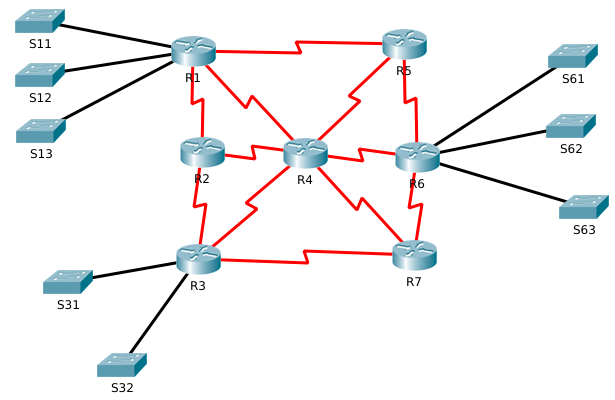
\includegraphics[scale=0.7]{iipac2018_is511_topologia_proyecto.png}
\end{figure}

\begin{table}[ht]
\centering
\caption{Requerimientos de direccionamiento}
\begin{tabular}{|c|c|c|}
\hline
\rowcolor[HTML]{C0C0C0} 
\#Empresa&Equipo asignado& Cantidad usuarios\\ \hline
    1   &S11   &    95 \\ \hline
   2    &S12   &   13  \\ \hline
      3 &S13   &    20   \\ \hline
    4   &S31   &   60                                       \\ \hline
    5 &S32    &     10                                     \\ \hline
     6    &S61          &    5                                      \\ \hline
         7   &S62  &      70                                    \\ \hline
         8   &S63       &    2                                      \\ \hline
\end{tabular}
\end{table}



\subsubsection{Tareas a realizar}
\begin{enumerate}
\item Definir estructura de direccionamiento, teniendo en cuenta que el espacio de direcciones es 172.16.0.0/16 para todas las redes LAN. Para conexiones WAN use bloques /30, a partir de 10.0.0.0
\item Implementar la topología de red. Utilice como base la que aparece en la Figura \# \ref{fig:fig_topology}. La cantidad de routers no debe ser modificada, tampoco sus conexiones.
%\item Implementar la topología diseñada en Packet Tracer v. 7.1
\item Documentar la asignación de direcciones IPv4 utilizando los ANEXOS 1 y 2.
\end{enumerate}

\subsection{Implementación de la topología}
\subsubsection{Packet Tracer v. 7.1}
\begin{enumerate}
\item Una vez realizado el diseño de la topología. Utilice el ANEXO 3 para el registro de los dispositivos.
\item Configurar el direccionamiento IPv4.
\item Configurar el DHCP en los routers que sea necesario. Utilice el ANEXO 5 para documentar dicha configuración.
\item Realizar la configuración de los parámetros básicos. Para el hostname utilice R o S, según corresponda seguido de un número, e.g. R1. Para el registro de contraseñas utilice el ANEXO 4.
\end{enumerate}

\subsubsection{Configuración de VLANs}
\begin{enumerate}
\item Configure las VLANs requeridas.
\item Haga el registro del VLAN ID, el nombre asignado y el propósito.
\end{enumerate}

\subsubsection{Configuración de enrutamiento dinámico}
Se utilizará el protocolo RIP, versión 2 para facilitar las tareas de enrutamiento de los equipos utilizados en el proyecto.

\subsubsection{Pruebas de conectividad}
\begin{enumerate}
\item Coloque un host en cada red. Configure la dirección IP que corresponda a la red donde ha sido conectado.
\item Realice pruebas de conectividad entre todos los hosts. Si no hay conectividad total, realice la resolución de problemas para encontrar y corregir errores.
\end{enumerate}


%%%%
\newpage
\section{ANEXO 1}
\noindent Nombre de empresa:\\
Espacio de direccionamiento:\\

\begin{table}[ht]
\centering
\caption{Registro de direccionamiento IPv4 -  LAN}
\begin{tabular}{|p{0.10\linewidth}|p{0.10\linewidth}|p{0.10\linewidth}|p{0.10\linewidth}|p{0.10\linewidth}|p{0.10\linewidth}|p{0.10\linewidth}|}
\hline
\rowcolor[HTML]{C0C0C0} 
\# subred & Dirección de red & Dirección de broadcast & Gateway & Máscara de subred & Espacio utilizado & Espacio libre            \\ \hline
          &                  &                        &         &                    &                   & \\ \hline
          &                  &                        &         &                    &                   & \\ \hline
          &                  &                        &         &                    &                   & \\ \hline
          &                  &                        &         &                    &                   & \\ \hline
\end{tabular}
\end{table}
%%%%

\section{ANEXO 2}
\begin{table}[ht]
\centering
\caption{Registro de direccionamiento IPv4 - WAN}
\begin{tabular}{|p{0.10\linewidth}|p{0.10\linewidth}|p{0.10\linewidth}|p{0.10\linewidth}|p{0.10\linewidth}|p{0.10\linewidth}|p{0.10\linewidth}|}
\hline
\rowcolor[HTML]{C0C0C0} 
\# subred & Router extremo 1 & Dirección IP & Router extremo 2 & Dirección IP\\ \hline
          &                  &                        &         &                     \\ \hline
          &                  &                        &         &                     \\ \hline
          &                  &                        &         &                    \\ \hline
          &                  &                        &         &                    \\ \hline
\end{tabular}
\end{table}

\section{ANEXO 3}
\begin{table}[ht]
\centering
\caption{Registro de equipo utilizado}
\begin{tabular}{|p{0.10\linewidth}|p{0.10\linewidth}|p{0.10\linewidth}|p{0.10\linewidth}|p{0.10\linewidth}|p{0.10\linewidth}|p{0.10\linewidth}|}
\hline
\rowcolor[HTML]{C0C0C0} 
Cantidad & Tipo de equipo & Modelo & \# y tipo de interfaces\\ \hline
          &                  &                        &               \\ \hline
          &                  &                        &                    \\ \hline
          &                  &                        &                   \\ \hline
          &                  &                        &                   \\ \hline
\end{tabular}
\end{table}
* tipo de equipo: router o switch

\section{ANEXO 4}
\begin{table}[ht]
\centering
\caption{Registro de contraseñas}
\begin{tabular}{|p{0.10\linewidth}|p{0.10\linewidth}|p{0.10\linewidth}|p{0.10\linewidth}|p{0.10\linewidth}|p{0.10\linewidth}|p{0.10\linewidth}|}
\hline
\rowcolor[HTML]{C0C0C0} 
Hostname & enable & línea de consola & línea VTY\\ \hline
          &                  &                        &               \\ \hline
          &                  &                        &                    \\ \hline
          &                  &                        &                   \\ \hline
          &                  &                        &                   \\ \hline
\end{tabular}
\end{table}

\section{ANEXO 5}
\begin{table}[ht]
\centering
\caption{Registro de rangos DHCP}
\begin{tabular}{|p{0.10\linewidth}|p{0.20\linewidth}|p{0.10\linewidth}|p{0.10\linewidth}|p{0.10\linewidth}|p{0.10\linewidth}|}
\hline
\rowcolor[HTML]{C0C0C0} 
Hostname & Rango de direcciones para DHCP & Dir. reservadas & Máscara de subred\\ \hline
          &                  &                        &               \\ \hline
          &                  &                        &                    \\ \hline
          &                  &                        &                   \\ \hline
          &                  &                        &                   \\ \hline
\end{tabular}
\end{table}
%%%%
%\newpage
\vfill
{\textbf {\normalsize José Mario López}}

{\small Profesor de la asignatura\\}

{\footnotesize 

\end{document}